\documentclass[11pt]{beamer}

\usetheme{metropolis}

\usepackage{graphicx}
\usepackage{physics}
\usepackage{adjustbox}
\usepackage{caption}
\usepackage{chemformula}
\usepackage{quoting}
\usepackage[style=chem-angew,backend=bibtex]{biblatex}
\bibliography{references}
%
% Choose how your presentation looks.
%
% For more themes, color themes and font themes, see:
% http://deic.uab.es/~iblanes/beamer_gallery/index_by_theme.html
%
\mode<presentation>
{
  \usetheme{default}      % or try Darmstadt, Madrid, Warsaw, ...
  \usecolortheme{default} % or try albatross, beaver, crane, ...
  \usefonttheme{default}  % or try serif, structurebold, ...
  \setbeamertemplate{navigation symbols}{}
  \setbeamertemplate{caption}[numbered]
  \setbeamerfont{footnote}{size=\tiny}
} 

\usepackage[english]{babel}
\usepackage[utf8]{inputenc}
\graphicspath{{../lectureMW/image}}

\AtBeginSection[]{
\begin{frame}{Outline}
  \tableofcontents[currentsection]
\end{frame}
}

\title{Chapter 9: Gaseous State}
\institute{Chemistry Department, Cypress College}
\date{Nov 29, 2022}

\begin{document}

\begin{frame}
  \titlepage
\end{frame}

\begin{frame}{Class Announcements}
  \textbf{Lecture}
  \begin{itemize}
  \item Return exam 3 and go over answers
  \item Begin Ch 9 and 10
  \item Quiz and Homework assignment released Fri, Dec
    2nd at 3pm
  \end{itemize}
\end{frame}

\section{Defining Gas Pressure}

\begin{frame}{Smokey the Bear: Hot Air Balloon}
  \begin{center}
    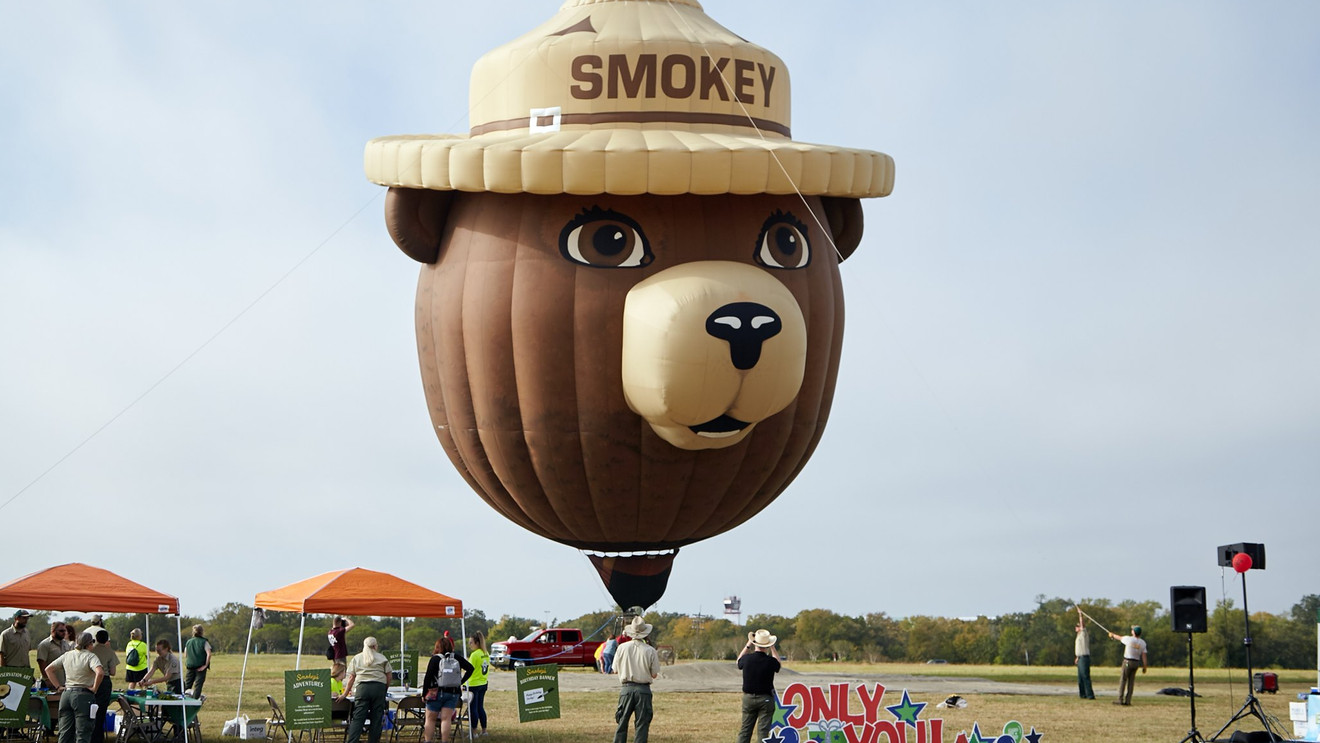
\includegraphics[scale=0.2]{smokey_air}
  \end{center}
  \textbf{Q:} How do air balloons float in the air?
\end{frame}

\begin{frame}{Defining Pressure}
  \begin{equation}
    P = \frac{F}{A}
  \end{equation}
  where $P$ is the pressure (N/m$^2$), $F$ is the force (Newton or N) acting on the area,
  and $A$ is the surface area (m$^2$)

  \textit{Common Units:} Psi, Torr, Pa, atm, mm Hg, and lb/in$^2$
\end{frame}

\begin{frame}{Measuring Pressure}
  \begin{center}
    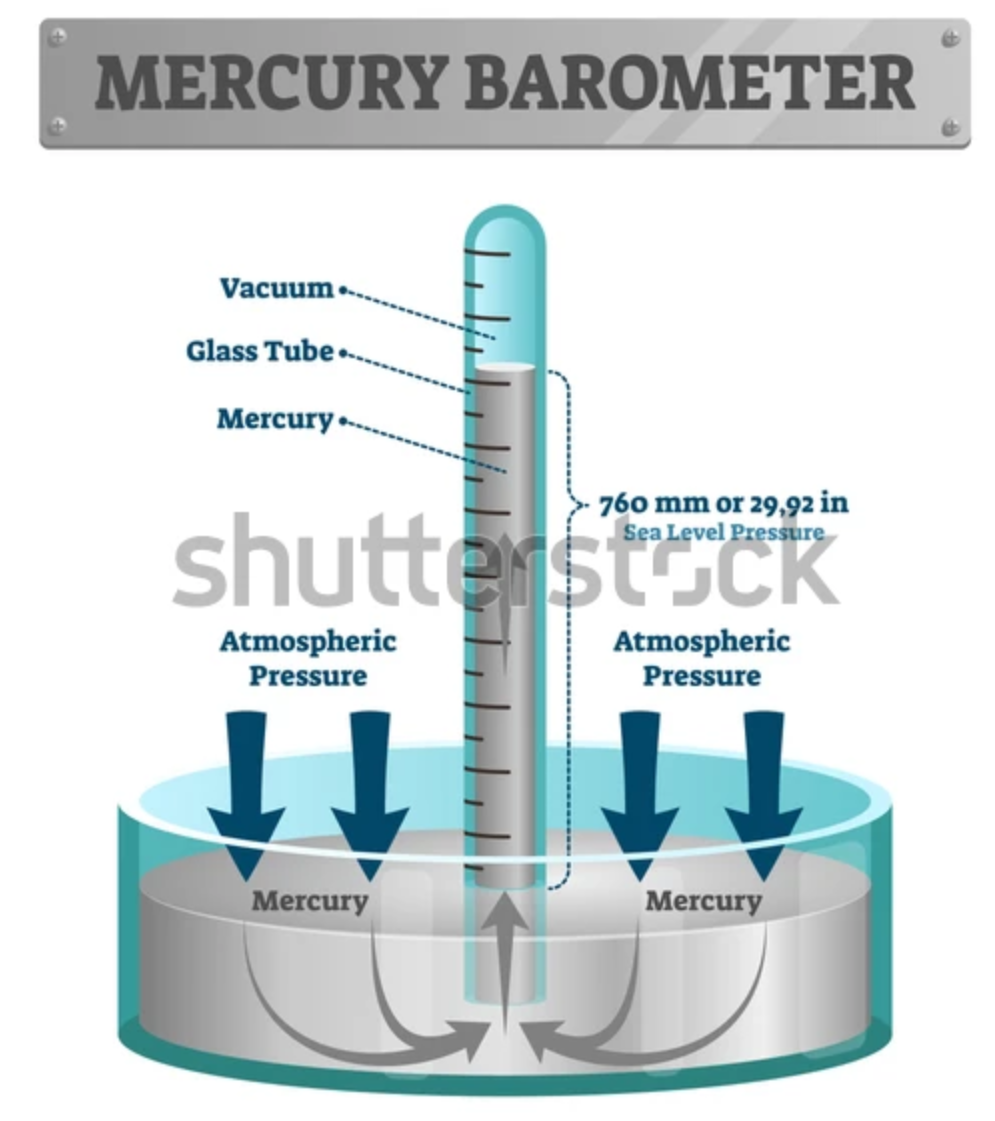
\includegraphics[width=0.6\linewidth]{merc_baro}
  \end{center}
\end{frame}

\begin{frame}{Common Pressure Units Conversion}
  \textit{Common Units:} Psi, Torr, atm, mm Hg, and lb/in$^2$
  \begin{align*}
    1 \text{atm} = & 760 \text{mm Hg} \\
    1 \text{atm} = & 101,325 \text{Pa} \\
    1 \text{atm} = & 14.7 \text{lb/in}^2
  \end{align*}
\end{frame}

\begin{frame}{Practice: Unit Conversion}
  Convert the following units:

  a) 845 Torr to atm

  b) 1.73 atm to Pa

  c) 32.1 lb/in$^2$ to atm

  \vspace{1in}
\end{frame}

\section{Gas Laws: Relationship P, V, and T}

\begin{frame}{Defn: Standard Temperature and Pressure}
  \textbf{Standard Temperature and Pressure (STP)}: the gas is at
  a given $0^\circ$C, 1 atm, and 22.414 L/mol
\end{frame}

\begin{frame}{Boyle's Law}
  For a given mole of gas, the pressure and volume are inversely
  proportional.
  \begin{align}
    PV = & \text{ constant} \\
    P_1V_1 = & P_2V_2
  \end{align}    
\end{frame}

\begin{frame}{Boyle's Law}
  \centering
  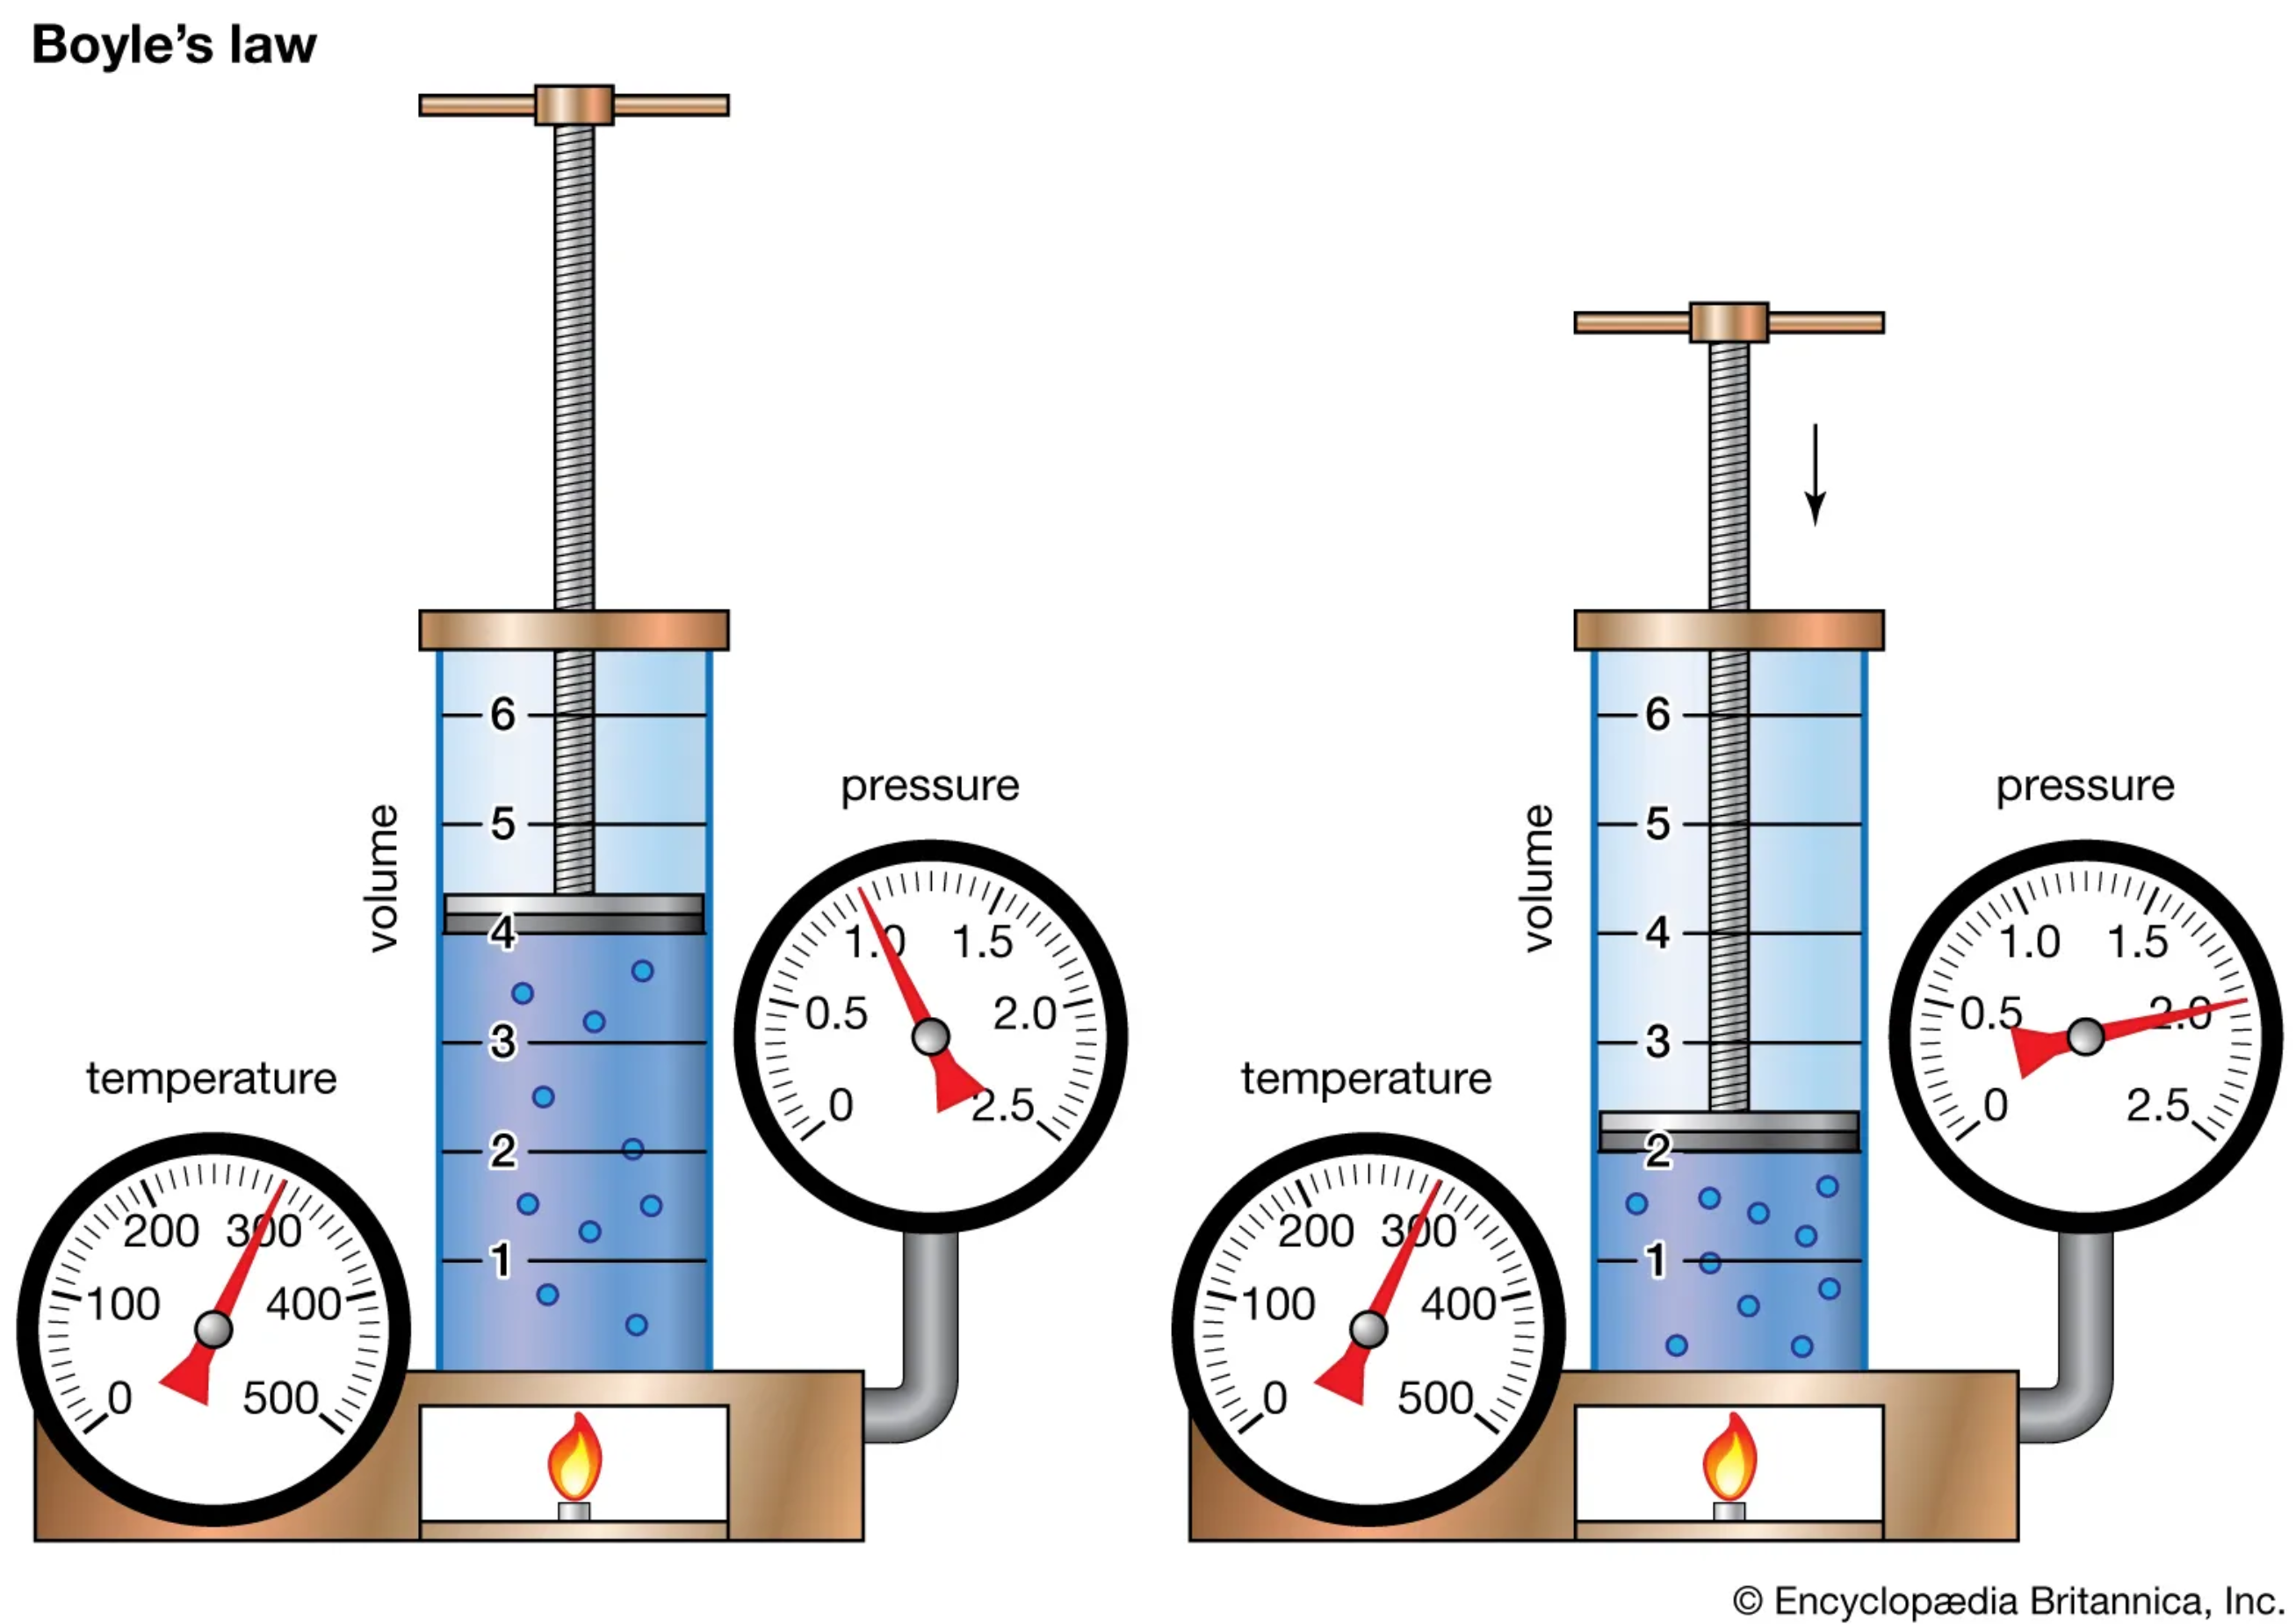
\includegraphics[width=\linewidth]{boyle_law}
\end{frame}

\begin{frame}{Graphing Boyle's Law}
  \centering
  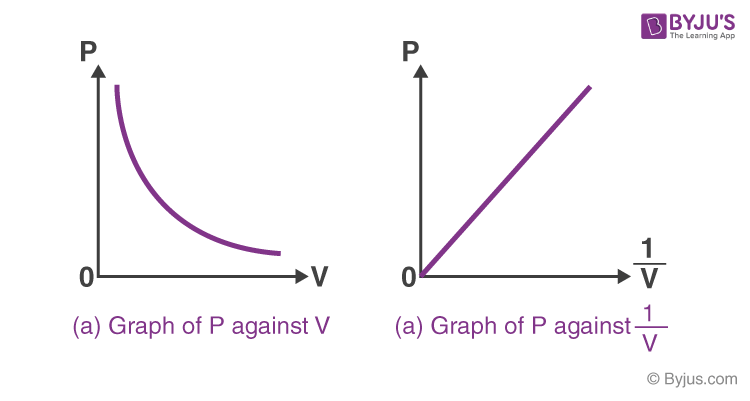
\includegraphics[width=0.9\linewidth]{boyle_graph}
\end{frame}

\begin{frame}{Practice: Boyle's Law}
  A balloon contains 510mL of helium when filled at 1.00atm. What would be
  the volume of the balloon if it were subjected to 2.50 atm of pressure?

  \vspace{1.5in}
\end{frame}

\begin{frame}{Charles' Law}
  For a given mole of gas, the volume and temperature are directly
  proportional
  \begin{align}
    \frac{V}{T} = & \text{ constant} \\
    \frac{V_1}{T_1} = & \frac{V_2}{T_2}
  \end{align}
  \textit{Note:} Temperature is in Kelvin! Conversion from $^\circ$C to
  K is defined:
  \begin{equation}
    K = {^\circ}C + 273.15
  \end{equation}
\end{frame}

\begin{frame}{Charles' Law}
  \centering
  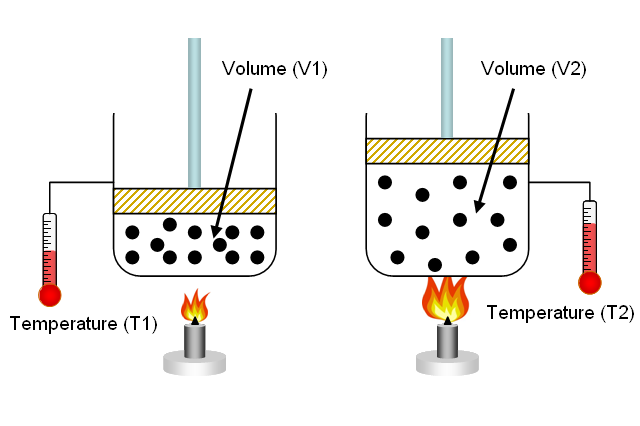
\includegraphics[width=0.9\linewidth]{charles_law}
\end{frame}

\begin{frame}{Graphing Charles' Law}
  \centering
  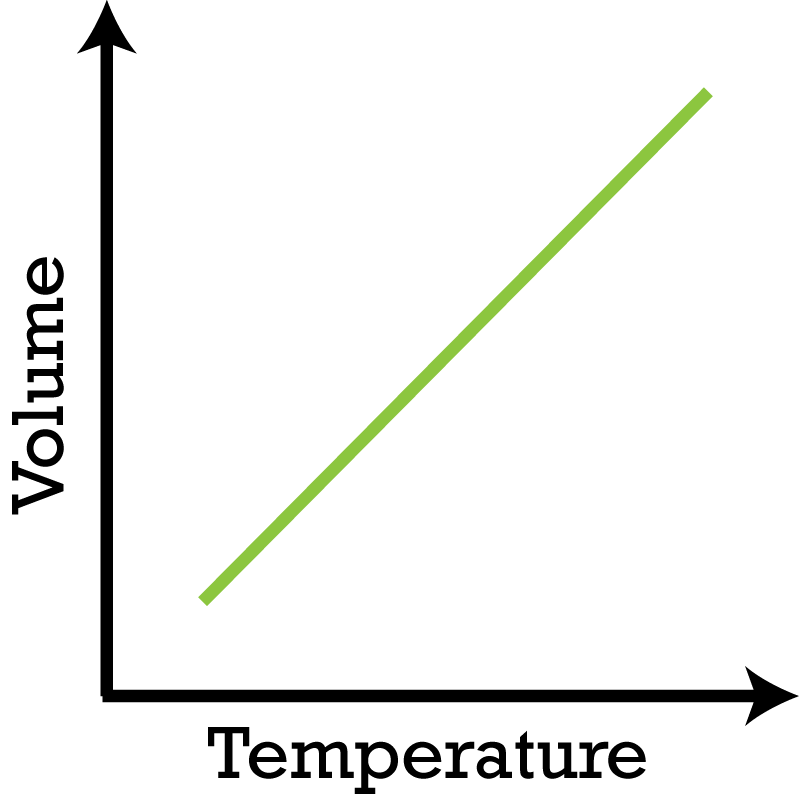
\includegraphics[width=0.6\linewidth]{charles_graph}
\end{frame}

\begin{frame}{Practice: Charles' Law}
  If a sample of chlorine gas occupies 50.0mL at 100.0$^\circ$C,
  what is its volume at 25.0$^\circ$C at constant pressure?
  
  \vspace{1.5in}
\end{frame}

\begin{frame}{Avogadro's Hypothesis}
  At constant temperature and pressure, the volume and moles of gas
  are directly proportional
  \begin{align}
    \frac{V}{n} = & \text{ constant} \\
    \frac{V_1}{n_1} = & \frac{V_2}{n_2}
  \end{align}
\end{frame}

\begin{frame}{Practice: Volume and Moles of Gas}
  If a 10.0L balloon contains 0.80 mol of a gas, what wil be the volume
  of a balloon that contains 0.20 mol of the gas if temperature and
  pressure remain constant?

  \vspace{1.5in}
\end{frame}

\section{Ideal Gas Law}

\begin{frame}{Greenhouse Effect}
  \centering
  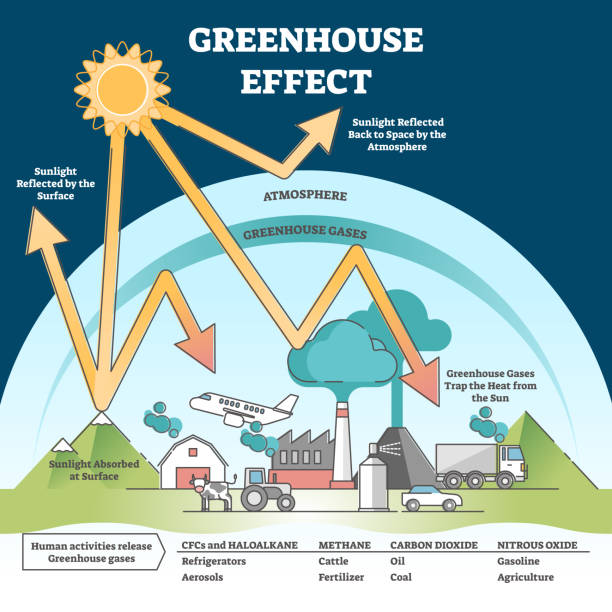
\includegraphics[width=\linewidth]{greenhouse_effect}
\end{frame}

\begin{frame}{Recall the Models}
  \textbf{Plum Pudding Model}
  \centering
  
  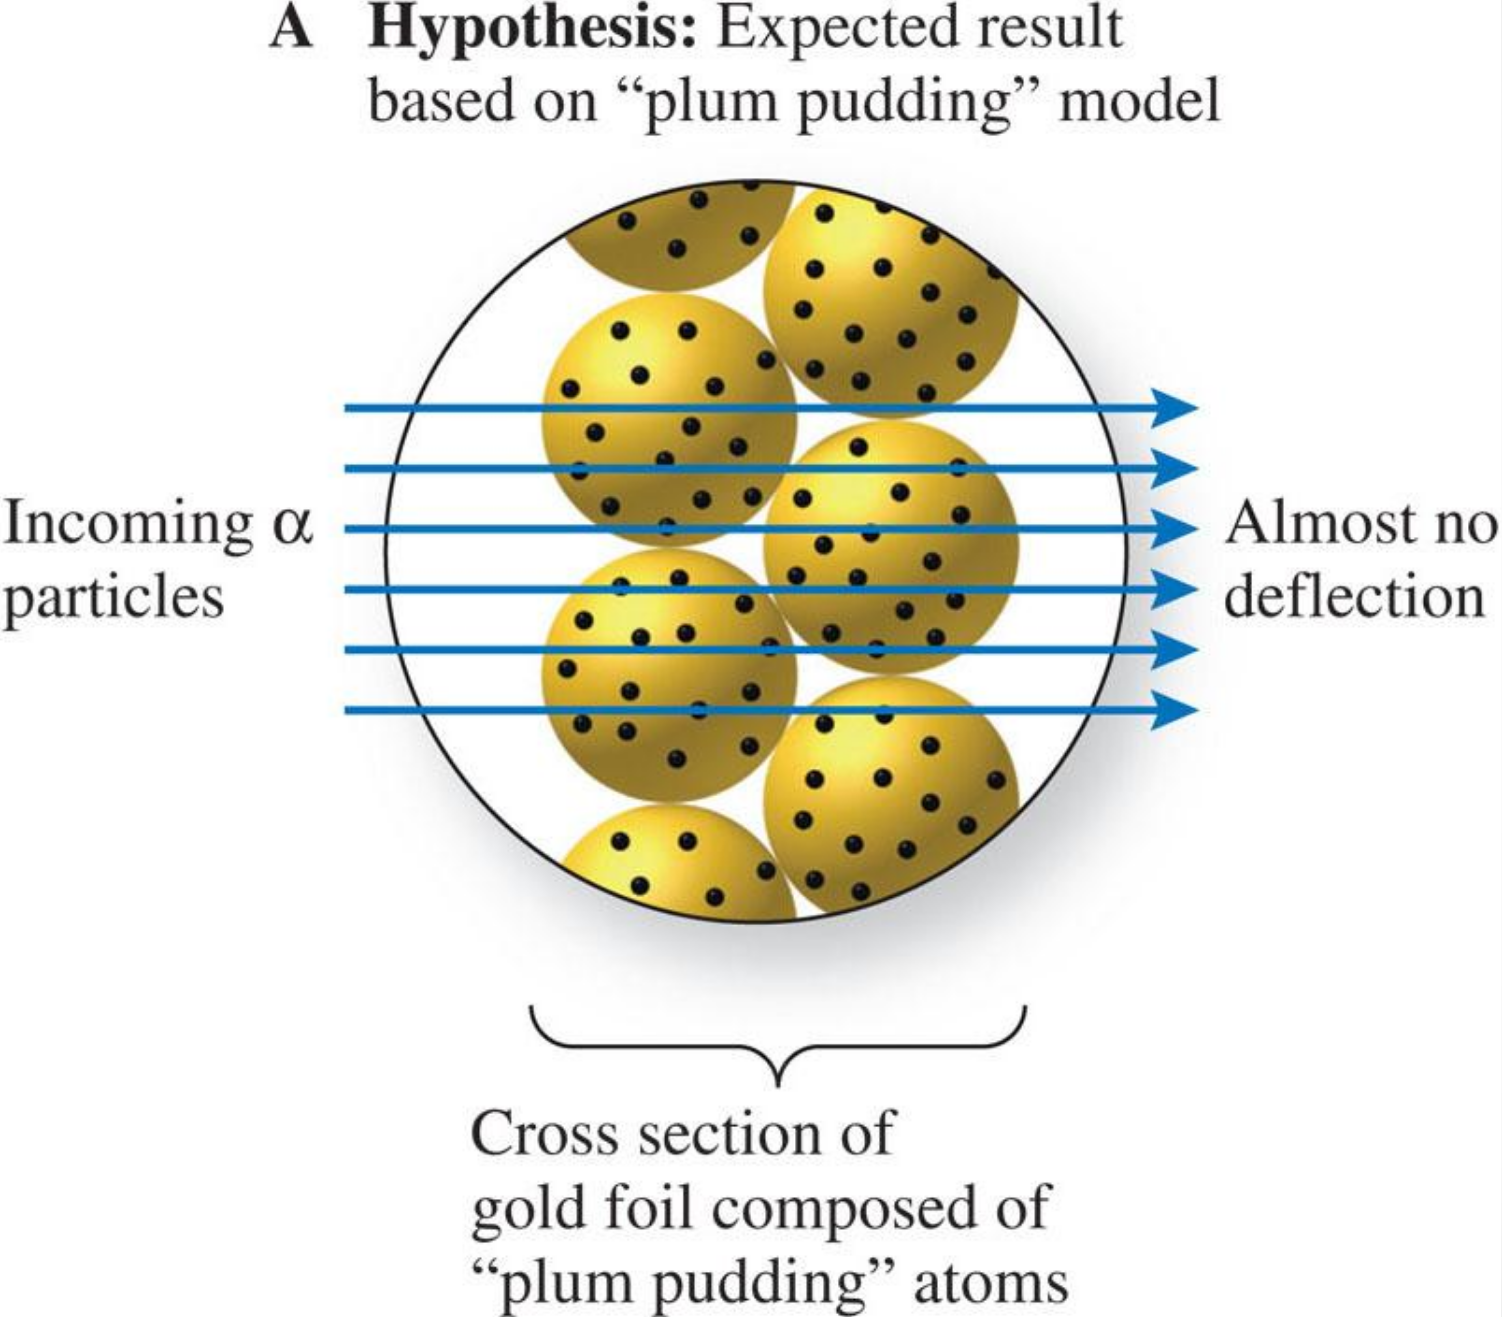
\includegraphics[width=0.7\linewidth]{test_hypothesis}
\end{frame}

\begin{frame}{Recall the Models}
  \centering
  \textbf{Bohr Model}

  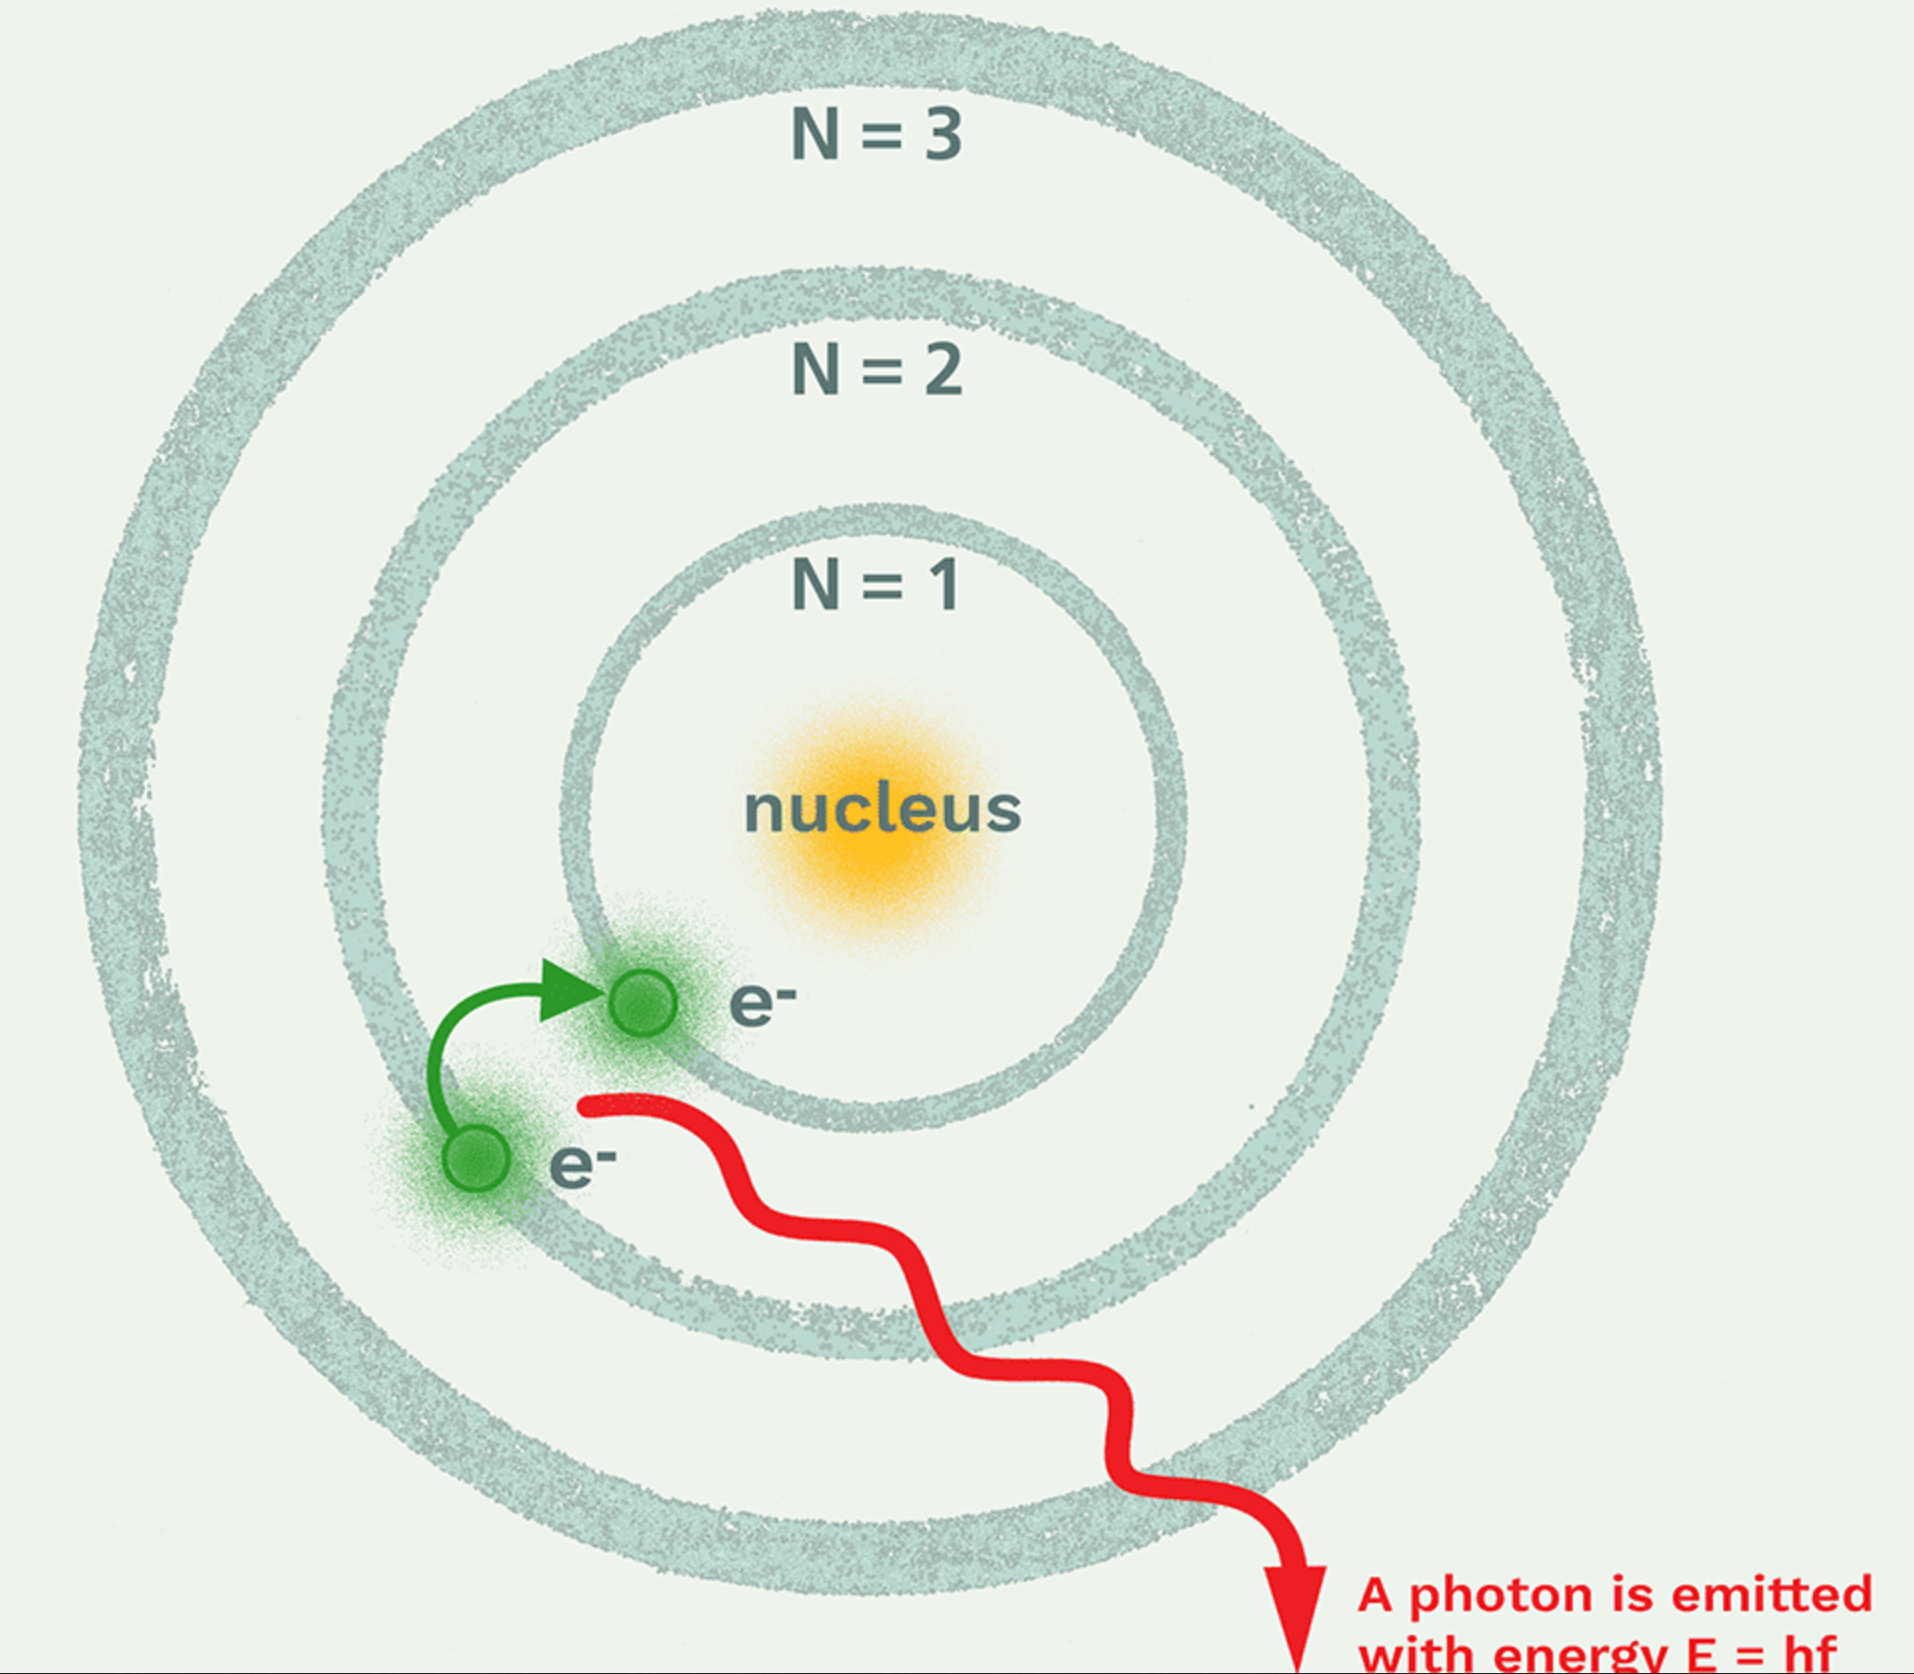
\includegraphics[width=0.7\linewidth]{bohr_model}
\end{frame}

\begin{frame}{Ideal Gas Model}
  \begin{equation}
    PV = nRT
  \end{equation}
  where $P$ is pressure (atm), $V$ is volume (L), $n$ moles of gas (mols),
  $R$ is gas constant, and $T$ is temperature (K)

  \onslide<2->{\textbf{Gas Constants} - Use the appropriate once based on the
  units in the problem
  \begin{align}
    R = & 8,314.46\,\frac{\text{L Pa}}{\text{K mol}}
    = 0.082057\,\frac{\text{L atm}}{\text{K mol}} \nonumber\\
    = & 62.3636\,\frac{\text{L Torr}}{\text{K mol}} \nonumber
  \end{align}
  }
\end{frame}

\begin{frame}{Using Ideal Gas to Obtain Gas Laws}
  \textbf{Boyle's Law} - hold $n$ and $T$ constant
  \onslide<2->{\begin{align}
    PV = & nRT \nonumber \\
    PV = & \text{constant} \\
    P_1V_1 = & P_2V_2 \nonumber
    \end{align}
  }
  \onslide<3->{\textbf{Charles' Law} - hold $n$ and $P$ constant}
  \onslide<4->{\begin{align}
    PV = & nRT \nonumber \\
    \frac{V}{T} = & \frac{nR}{P} = \text{constant} \\
    \frac{V_1}{T_1} = & \frac{V_2}{T_2} \nonumber
    \end{align}
  }
\end{frame}

\begin{frame}{Practice: Avogadro's Hypothesis}
  Obtain the Avogadro's hypothesis formula from the ideal gas law
  ($PV = nRT$).
  \vspace{1in}
\end{frame}

\begin{frame}{Practice: Using Ideal Gas}
  Assuming ideal gas, what is the temperature for 2.10 moles of N$_2$ gas under
  1.25 atm and in 25.0 L? ($R=0.082057$ (L atm)/(K mol))
  \vspace{1in}
\end{frame}

\begin{frame}{Practice: Using Ideal Gas}
  The volume of a propane cylinder is 0.960L. When filled, the cylinder contains
  liquid propane stored under pressure. When the cylinder is ``empty,'' it contains
  propane gas molecules at atmospheric ppressure and temperature. How many
  moles of propane gas remain in a cylinder when it is empty if the surrounding
  atmospheric conditions are 298K and 0.980atm.
  \vspace{1.2in}
\end{frame}

\begin{frame}{Finding Density from Ideal Gas Law}
  \textbf{Q:} What are the units for density?
  \onslide<2->{\begin{align*}
      PV = & nRT \\
      \frac{n}{V} = & \frac{P}{RT}
    \end{align*}
    Given this ratio, the last step is to multiply by the molar
    mass of the given substance
  }
  \onslide<3->{\begin{align*}
      D = \frac{n\,MM}{RT}
    \end{align*}
    where $MM$ is the molar mass
  }
\end{frame}

\begin{frame}{Practice: Determine Density from Ideal Gas}
  Calculate the density of butane at 298.15K and a pressure of
  0.987atm. The gas constant is 0.08206 (L atm)/(K mol). %2.35 g/L
  \vspace{1.5in}
\end{frame}

\section{Dalton's Law of Partial Pressures}

\begin{frame}{Dalton's Law of Partial Pressures}
  Gases in a mixture behave independently and exert the same pressure they would
  exert if they were in a container alone
  \begin{equation}
    P_\text{Total} = P_A + P_B + P_C + \cdots
  \end{equation}
  where $P_\text{Total}$ is the total pressure and $P_A, P_B, \cdots$ are the
  pressures of the components
\end{frame}

\begin{frame}{Dalton's Law of Partial Pressures}
  \begin{center}
    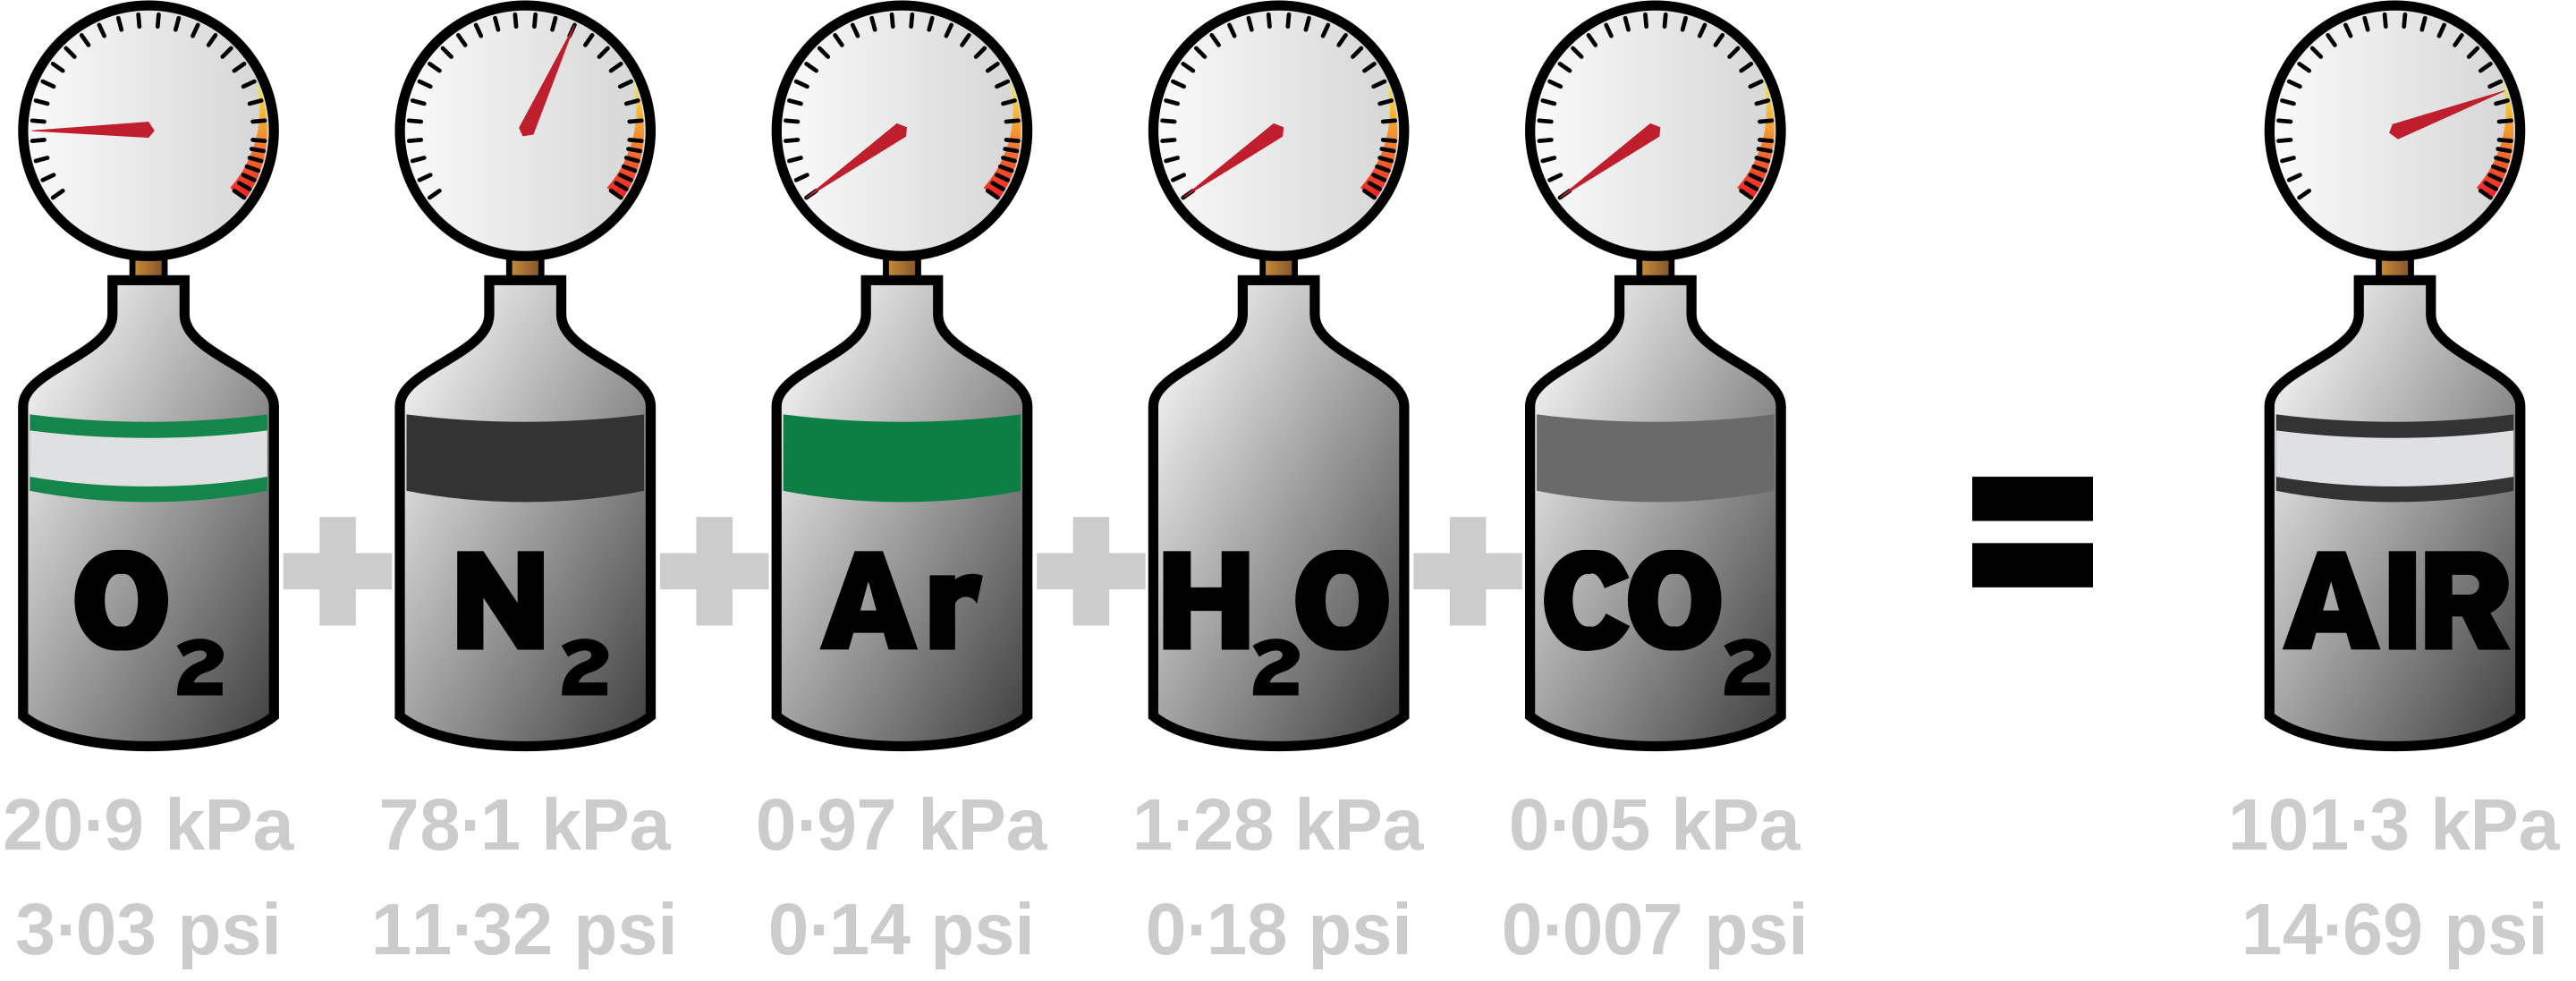
\includegraphics[width=\linewidth]{dalton_partial}
  \end{center}
  \begin{equation}
    P_\text{Total} = P_\text{O2} + P_\text{N2} + P_\text{Ar}
    + P_\text{H2O} + P_\text{CO2}
    \nonumber
  \end{equation}
\end{frame}

\begin{frame}{Practice: Dalton's Law of Partial Pressure}
  Suppose gaseous oxygen (O$_2$) is produced by:

  2KClO$_3$(s) $\rightarrow$ 2KCl(s) + 3O$_2$(g)

  If 1.50L of O$_2$ is collected over water at 300.K and 0.970atm,
  how many moles of O$_2$ is produced? The vapor pressure of water
  is 0.0351atm.
  \vspace{1.3in}
\end{frame}

\end{document}
